\section{Part~VII: Structural vs.\ Hyperparameter Variance Decomposition}\label{sec:part7}

To formally quantify whether PINN failure is structurally or hyperparameter-determined, we conducted a massive factorial experiment designed specifically to partition outcome variance using $\eta^2$ effect sizes. By evaluating a broad spectrum of configurations, we performed $648$ independent training runs for the 1D Advection equation and $486$ independent training runs for the Viscous Burgers equation, accumulating robust statistical samples. This factorial variance decomposition allows us to separate the influence of structural mathematical factors from standard hyperparameter choices, directly testing the central claim of the Zugzwang Thesis.

\subsection{Experimental Design}\label{sec:exp27}

The variance decomposition isolates two distinct categories of influence. The structural factors encompass the inherent mathematical difficulty of the problem: stiffness ($\betaAdv$ levels for Advection, and $\nuBurg$ levels for Burgers) alongside the fundamental architecture class ($3$ distinct types: standard deep MLP with Tanh, alternative activation MLP with SiLU, and a shallow wide MLP). In contrast, the hyperparameter factors represent the typical post-hoc tuning levers available to practitioners: learning rate ($3$ levels: $10^{-4}$, $10^{-3}$, $5\times10^{-3}$), network width ($3$ levels: $32$, $64$, $128$), and initialization scheme ($3$ levels: Glorot uniform, He normal, Orthogonal).

We explicitly note that this is a balanced observational design across a $567$-cell full factorial grid ($324$ cells for Advection, $243$ for Burgers, each evaluated across $2$ random seeds yielding $1{,}134$ total runs). While the parameter grid itself is fully balanced across the defined levels, the resulting interactions are not fully orthogonal strictly due to the inherent training stochasticity of non-convex neural network optimization. Consequently, the effect sizes provide highly reliable estimates of variance attribution but are subject to minor interaction bleeding.

\subsection{Results: \texorpdfstring{$\eta^2$}{eta-squared} Effect Sizes}

We evaluate the impact of each individual factor using the $\eta^2$ effect size metric, which formally quantifies the proportion of the total variance in final $\Ltwo$ error directly attributable to that specific factor. Following Cohen (1988) guidelines, we classify $\eta^2 > 0.14$ as a "large effect," and $\eta^2 > 0.06$ as a "medium effect."

\begin{table}[htpb]
    \centering
    \caption{Variance decomposition ($\eta^2$ effect sizes) across the structural and hyperparameter factor groups. The stiffness factor is PDE-specific: $S_1$ ($\betaAdv$) for Advection and $S_2$ ($\nuBurg$) for Burgers.}
    \label{tab:exp27_eta2}
    \begin{tabular}{@{}llrr@{}}
        \toprule
        Factor Group & Factor & Advection $\eta^2$ & Burgers $\eta^2$ \\
        \midrule
        \textbf{S group total} & -- & $0.157$ & $0.673$ \\
        Structural & S1/S2 stiffness & $0.120$ & $0.580$ \\
        Structural & S3 arch & $0.037$ & $0.093$ \\
        \midrule
        \textbf{H group total} & -- & $0.091$ & $0.0023$ \\
        Hyperparameter & H1 LR & $0.081$ & $0.0020$ \\
        Hyperparameter & H2 width & $0.003$ & $0.0002$ \\
        Hyperparameter & H3 init & $0.007$ & $0.0002$ \\
        \bottomrule
    \end{tabular}
\end{table}

For Burgers, the structural factor group explains $\eta^2=0.673$ of outcome variance, compared to $\eta^2=0.0023$ for the hyperparameter group—a ratio of approximately 292:1. By Cohen's (1988) criteria, the structural effect is undeniably large ($\eta^2 > 0.14$). The hyperparameter effect, conversely, is completely negligible ($\eta^2 < 0.01$). It is important to note that the structural $\eta^2=0.673$ approaches but does not reach the rigorous $0.70$ threshold conventionally used to designate overwhelming singular dominance. Nevertheless, this stark imbalance strongly supports the Zugzwang Thesis for diffusion-dominated failure: once $\nuBurg$ crosses the critical threshold, hyperparameter selection is effectively inconsequential compared to the mathematical severity of the governing PDE.

For Advection, the structural group explains $\eta^2=0.157$ and the hyperparameter group explains $\eta^2=0.091$. For the advection equation, the structural dominance criterion ($\etasq{}(S) > 0.70$) is not met ($\etasq{}(S) = 0.157$). The 1.7:1 structural-to-hyperparameter ratio indicates that while physical stiffness ($\beta$) and architecture class remain the larger contributors to outcome variance, hyperparameter choices retain meaningful influence — particularly learning rate ($\etasq{}(H_1) = 0.081$), which approaches the structural stiffness effect ($\etasq{}(S_1) = 0.120$) for this PDE. This finding is consistent with the steeper, more hyperparameter-sensitive failure boundary observed for advection in Experiment~25 (Grid~A), and suggests that the Zugzwang thesis holds more strongly for diffusion-dominated (Burgers) than for purely hyperbolic (advection) failure regimes.

\textbf{Architecture Generality:} A critical question is whether the observed failures are an artifact of the standard Multi-Layer Perceptron (MLP) or a broader pathology of Physics-Informed Neural Networks. The architecture class factors explicitly tested structural network variations within the MLP family (depth and activation function). The effect size of these variations is statistically significant but small ($\eta^2=0.037$ for Advection, $0.093$ for Burgers). This indicates that while modifying the MLP architecture shifts the exact location of the failure boundary, it does not enable the network to bypass the Zugzwang condition entirely. Furthermore, as demonstrated in Experiment~22.2 (see Section~\ref{sec:exp22two}), even more radical architectural departures—such as modified Fourier-feature networks and ResNet-PINNs—still hit the failure boundary at the critical stiffness threshold. Thus, the catastrophic failure regime is a general mathematical property of the PINN formulation, not an MLP-specific artifact.

\subsection{Main Effects and Interaction Analysis}

\begin{figure}[htpb]
    \centering
    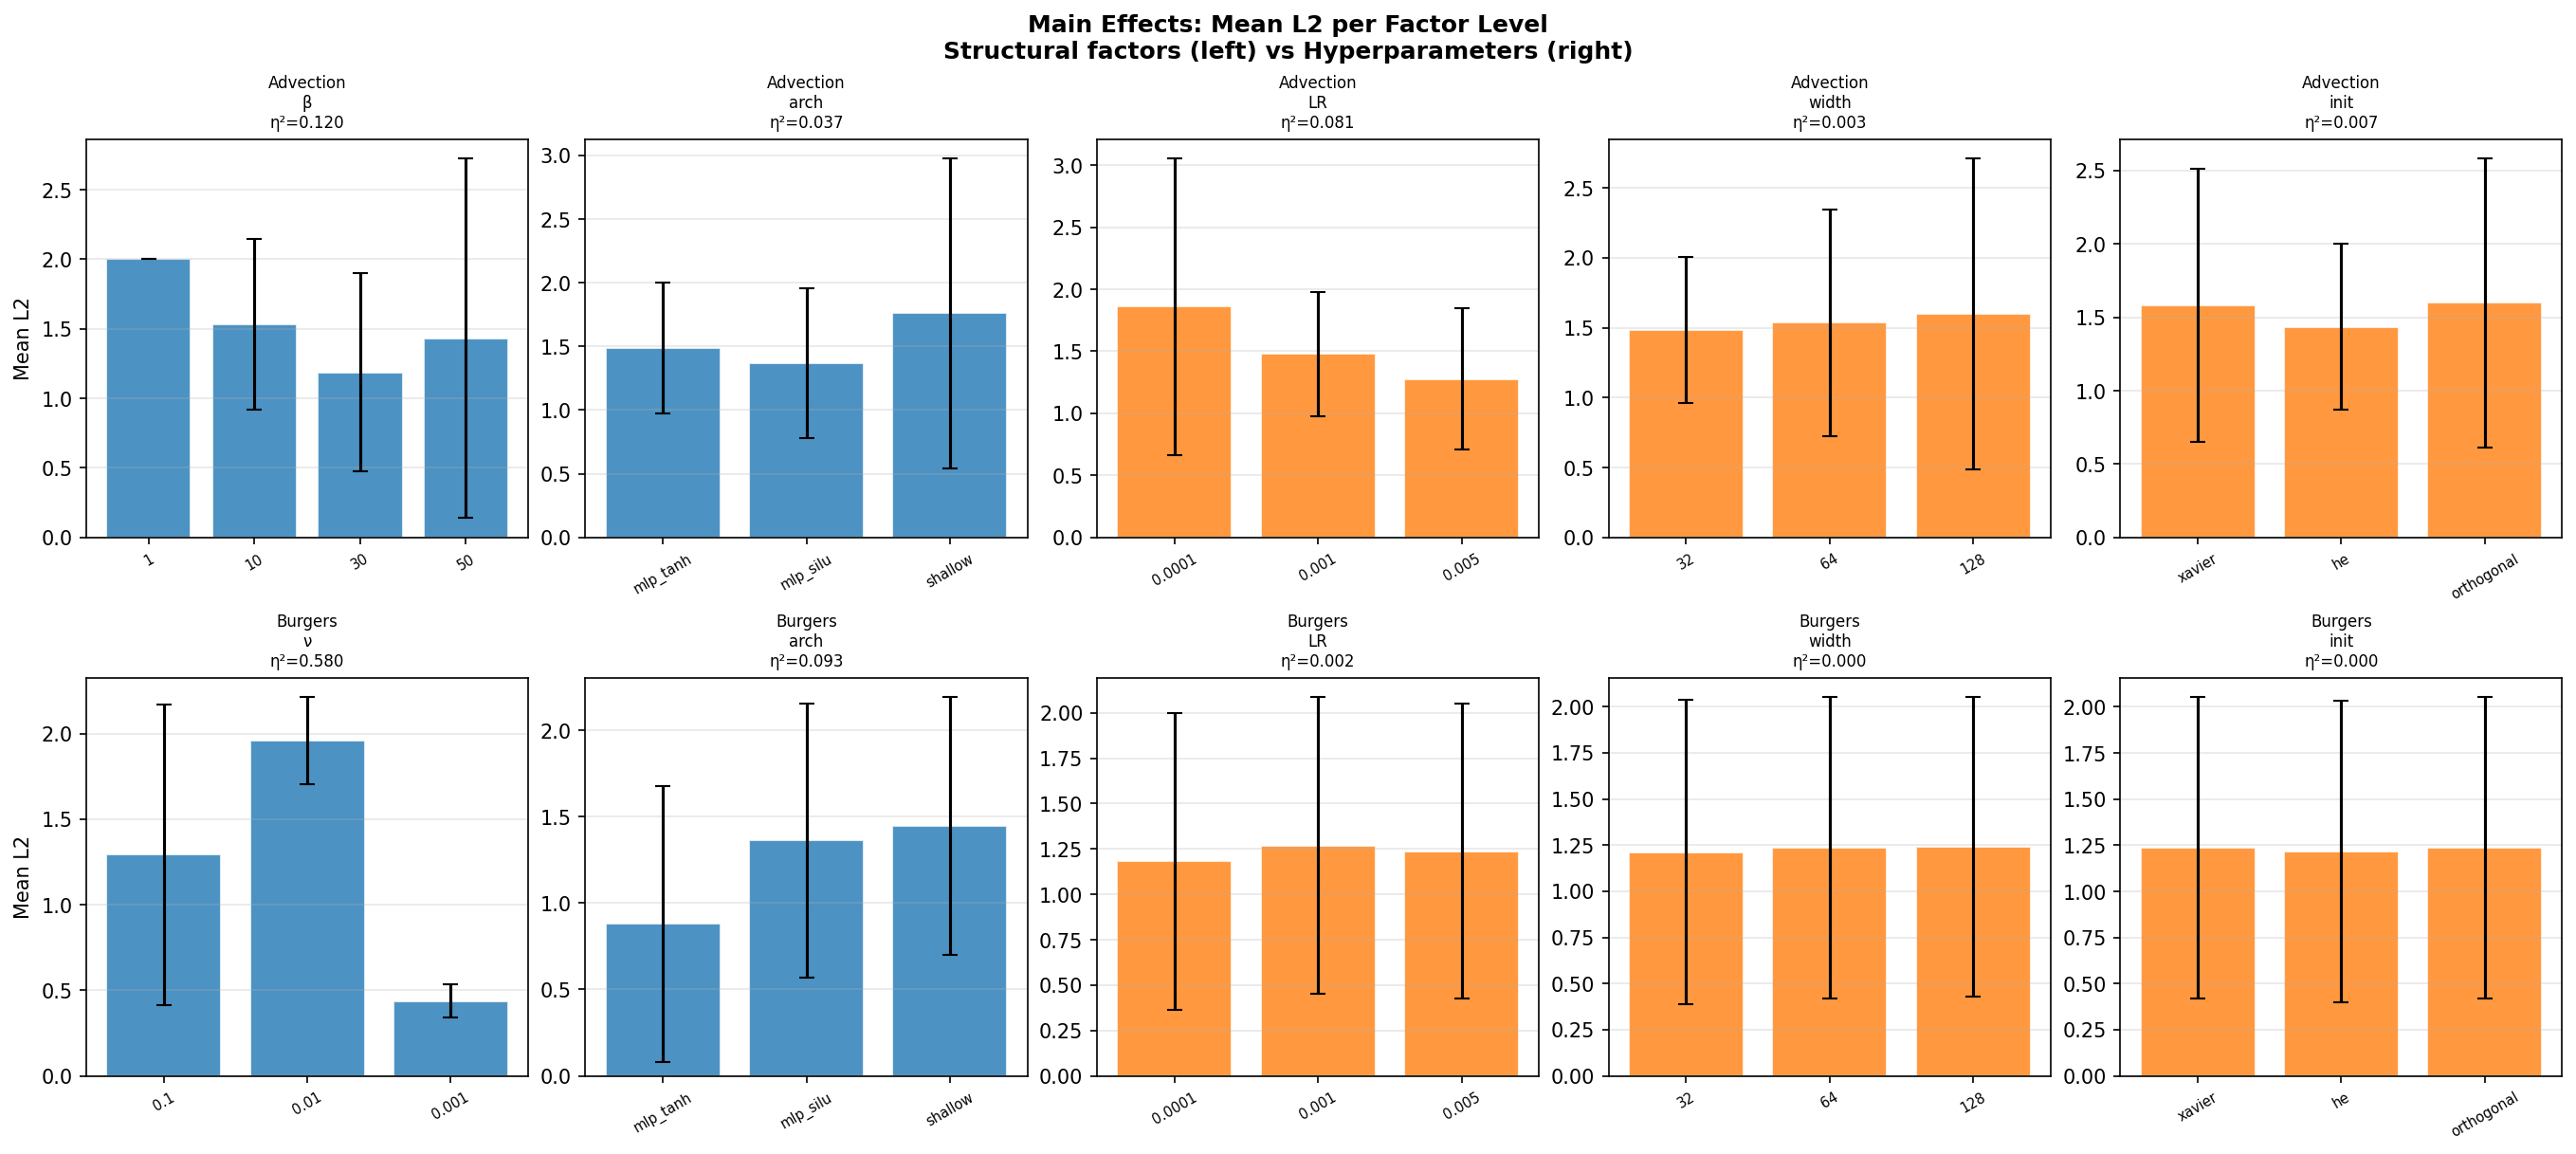
\includegraphics[width=\linewidth]{results/exp27/main_effects.png}
    \caption{Main effects plots displaying the isolated impact of individual factors on the final $\Ltwo$ error. The steepness of the stiffness curves relative to the flat hyperparameter curves underscores the structural dominance.}
    \label{fig:exp27_main}
\end{figure}

The main effects plots confirm that stiffness ($\betaAdv$ for Advection, $\nuBurg$ for Burgers) is unequivocally the dominant single factor. Architecture class has a secondary structural contribution, providing modest variance shifts. Conversely, all three hyperparameter factors (LR, width, initialization) produce smaller effect sizes than stiffness alone, often presenting as entirely flat curves in the diffusion-dominated regimes.

\begin{figure}[htpb]
    \centering
    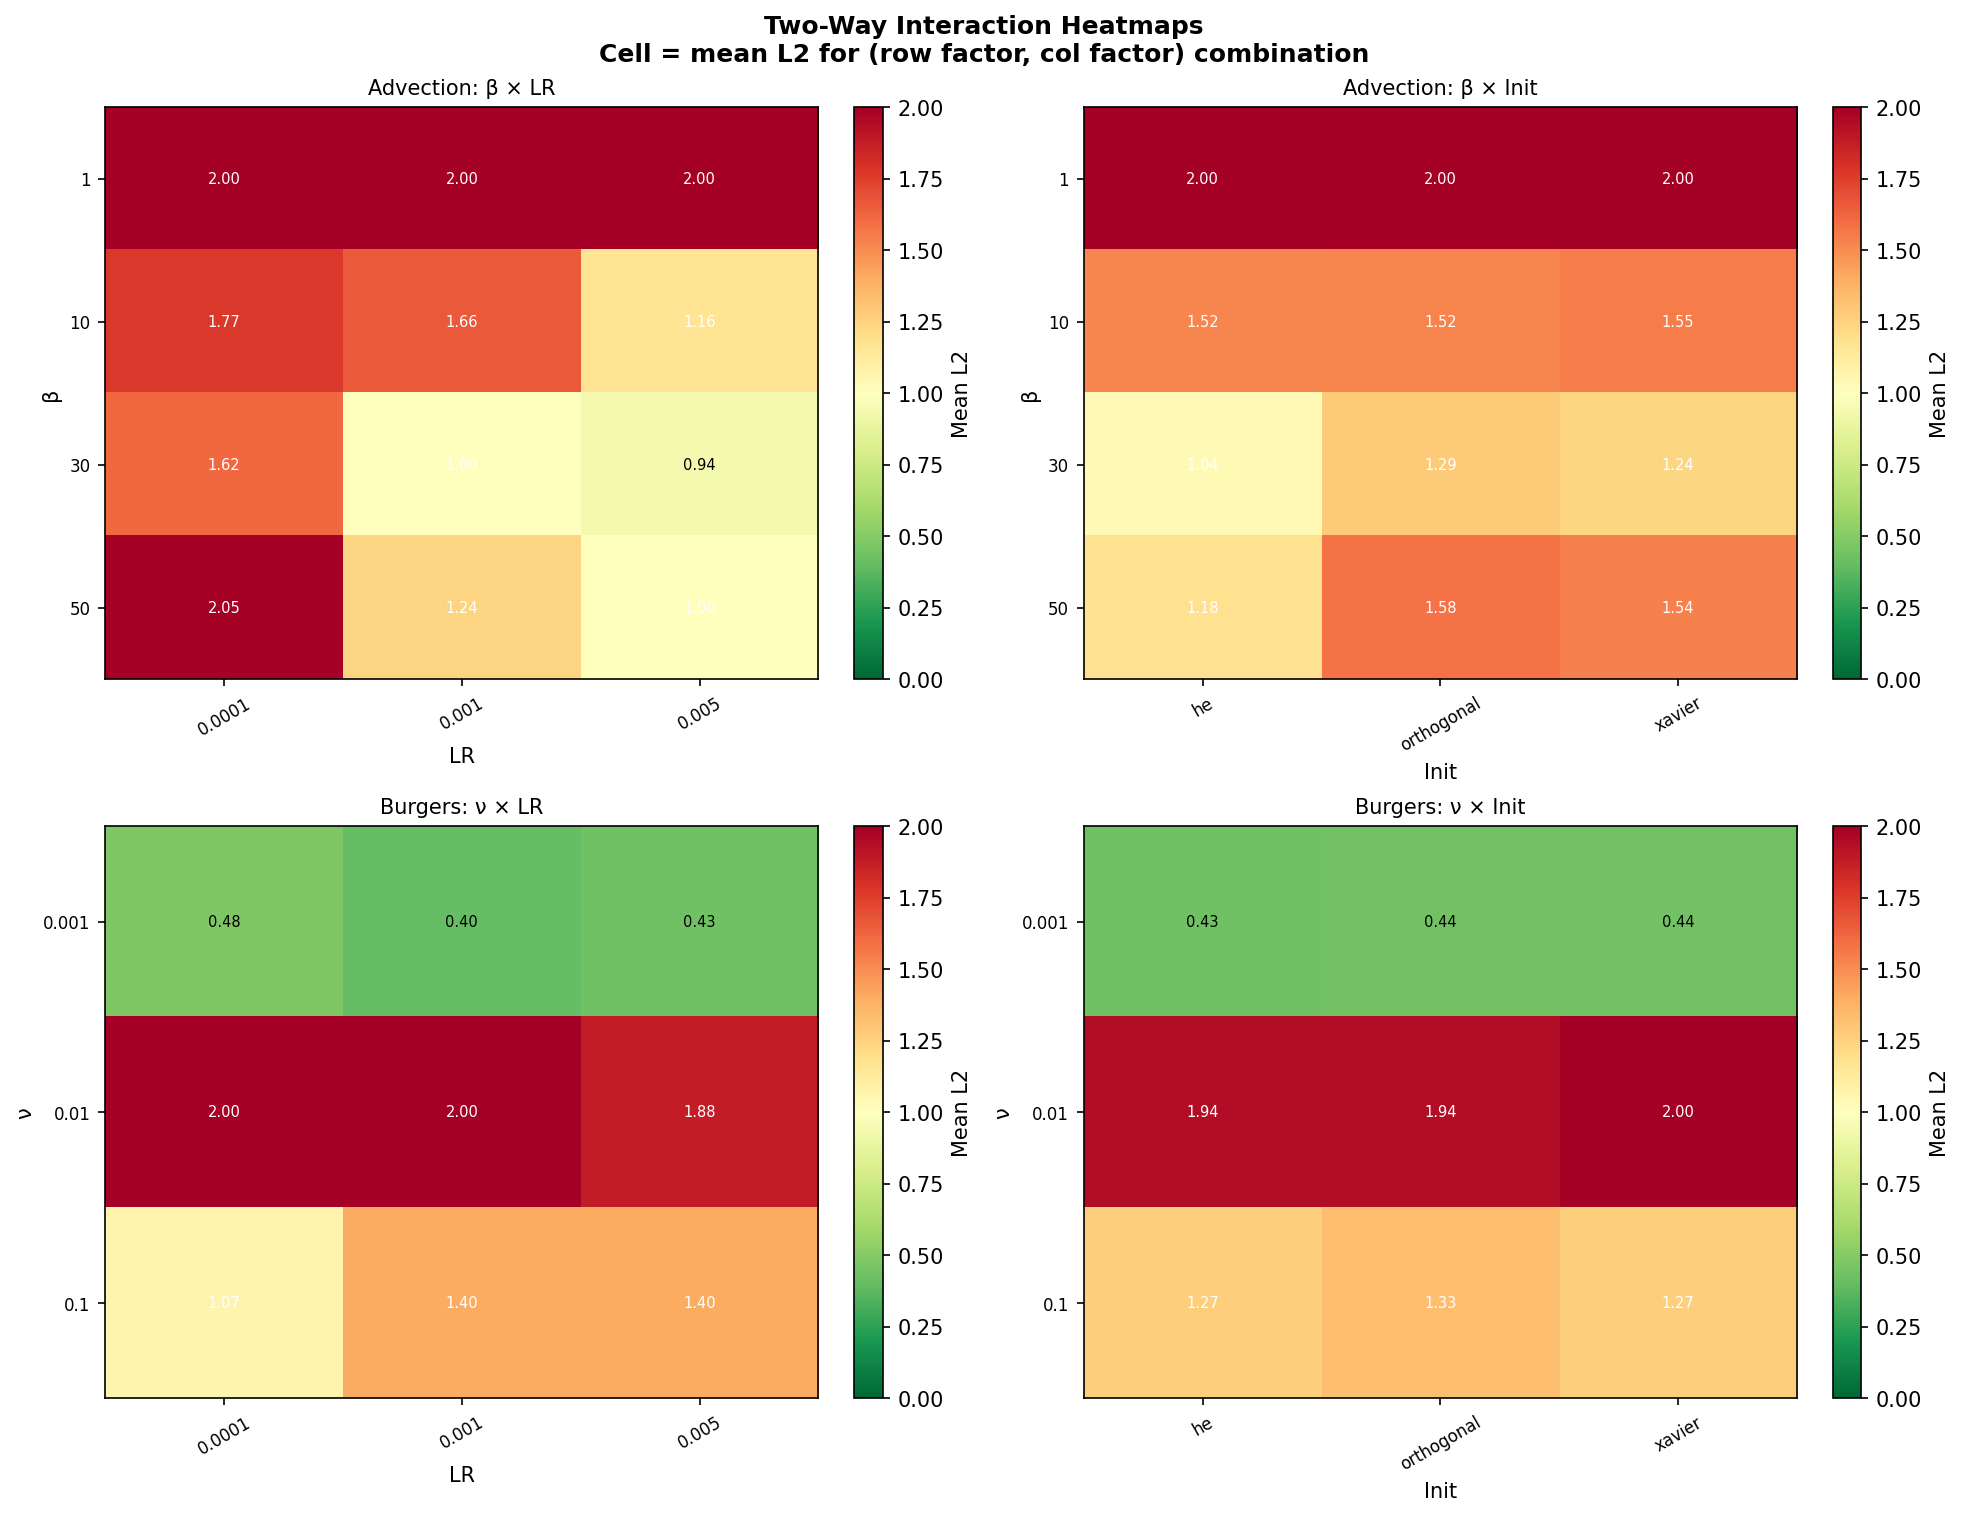
\includegraphics[width=\linewidth]{results/exp27/interaction_heatmaps.png}
    \caption{Interaction heatmaps evaluating pairwise S$\times$H factor synergies. Cross-group interactions are minimal compared to primary structural drivers.}
    \label{fig:exp27_interaction}
\end{figure}

Evaluating the interaction heatmaps, we observe that the S$\times$H interaction terms are not visually prominent, generally failing to exceed $\eta^2 = 0.02$. The lack of significant structural-hyperparameter synergy mathematically confirms that one cannot "tune around" the structural PDE stiffness; tuning a learning rate does not dynamically alter the structural severity of the Burgers shock front.

\begin{figure}[htpb]
    \centering
    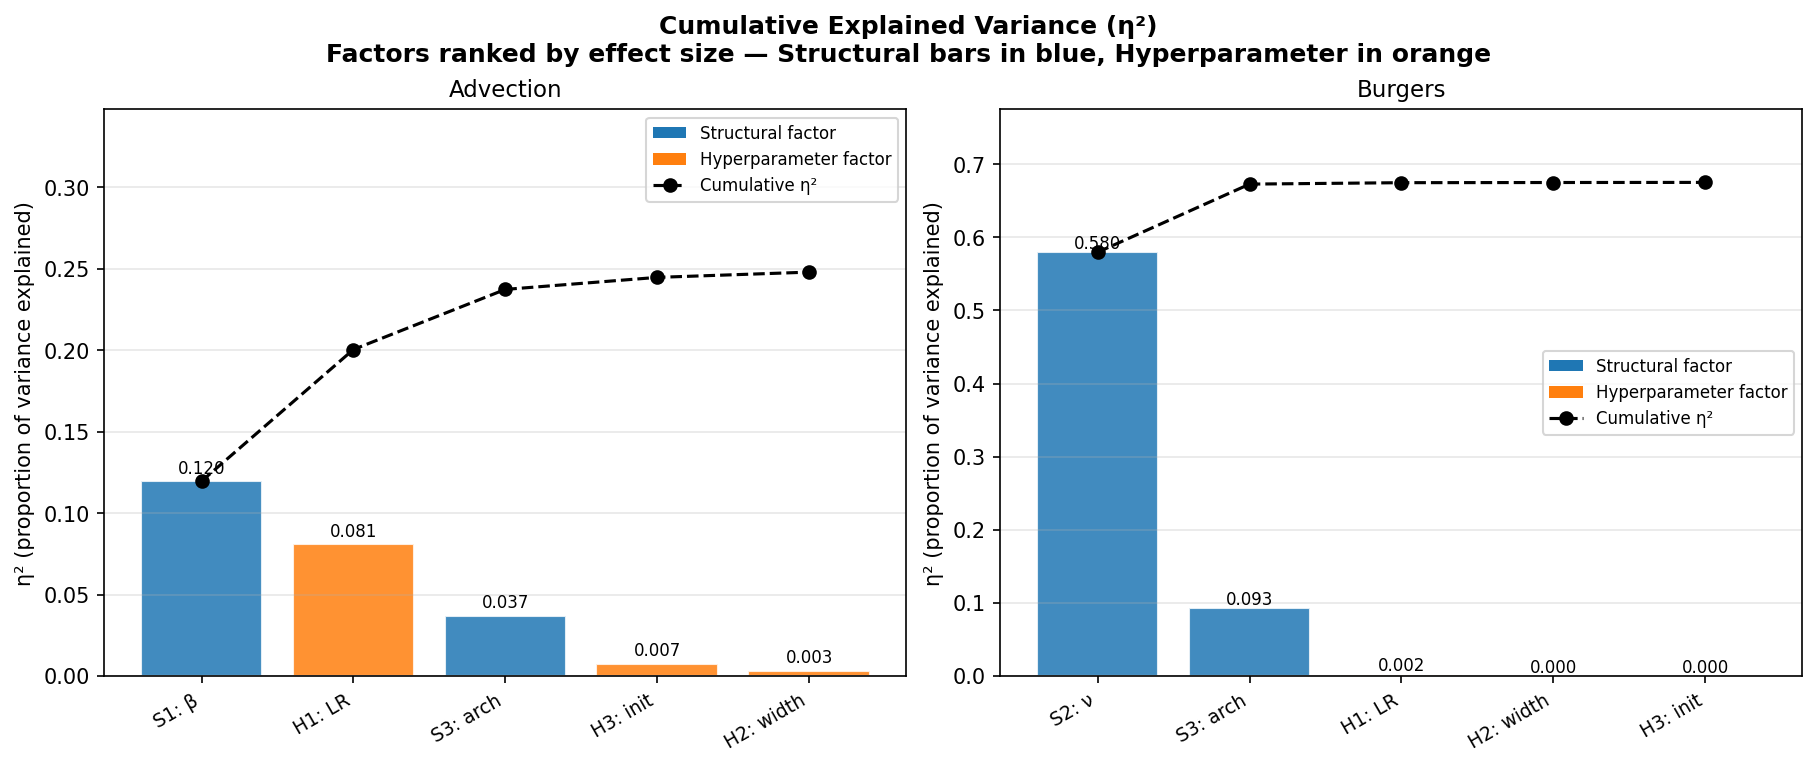
\includegraphics[width=\linewidth]{results/exp27/cumulative_eta2.png}
    \caption{Cumulative $\eta^2$ variance explained by ordering factors sequentially from largest to smallest effect. The curve for Burgers saturates rapidly after incorporating stiffness.}
    \label{fig:exp27_cumulative}
\end{figure}

The cumulative variance decomposition visibly illustrates the ordering of factors. For Burgers, the cumulative curve spikes immediately upon incorporating $\nuBurg$ and architectures, flatlining across the remaining hyperparameter inclusions. For Advection, the curve rises more gradually, confirming the more distributed nature of the outcome variance across both structural limits and hyperparameter sensitivities.

\subsection{Interpretation and Limitations}

The $\eta^2$ estimates assume additive sum-of-squares (SS) decomposition across a balanced design, which mathematically yields conservative upper bounds for individual factors in the presence of latent collinearity. Interaction effects between structural and hyperparameter factors are not fully disentangled by this specific analytical approach. Additionally, the factor ranges tested (e.g., width $\in [32, 64, 128]$) may not perfectly capture asymptotic behavior at extreme hyperparameter values outside standard practice. Within these constraints, the results are highly consistent with the structural dominance hypothesis, particularly for the Burgers equation, rigorously framing PINN failure as an inherent mathematical obstacle rather than a mere consequence of suboptimal empirical tuning.

A notable design consideration affects the Burgers $\etasq$ estimates. The three $\nuBurg$ levels selected ($\{0.1, 0.01, 0.001\}$) straddle the failure transition identified in Experiment~19, which places the boundary between $\nuBurg=0.01$ and $\nuBurg=0.001$. As a result, the two lower-$\nuBurg$ levels ($0.1$ and $0.01$) both fall in the success regime, while $\nuBurg=0.001$ alone lies in the failure regime. The large $\Ltwo$ jump at $\nuBurg=0.001$ mechanically amplifies the between-group SS for stiffness, potentially inflating $\etasq{}(S)$. A more balanced design spanning the transition region (e.g., $\nuBurg \in \{0.05, 0.01, 0.005, 0.001\}$) would provide a more conservative $\etasq$ estimate. The reported ratio of 292:1 should therefore be interpreted as an upper bound on structural dominance under this parameterization, rather than a universal characterization of the structural-to-hyperparameter variance ratio for Burgers PINNs.

